\subsection{PID-Regler}
Der PID-Regler (Proportional-Integral-Derivativ) ist eine weit verbreitete Regelungsstrategie in industriellen Steuerungssystemen und verschiedenen Arten von Anwendungen. Er ist unerlässlich für die Regelung von Prozessen wie Geschwindigkeit, Temperatur und Spannung~\cite[p.~2]{Hussein2011PIDGA}.

\paragraph{Proportionalanteil (P)}
Diese Komponente erzeugt einen Ausgangswert, der proportional zum aktuellen Fehlerwert ist. Die proportionale Reaktion kann durch Multiplikation des Fehlers mit einer Konstanten namens \( K_p \) eingestellt werden, die als Proportionalverstärkung bezeichnet wird.
\begin{equation}
P_{\text{out}} = K_p \times e(t)
\end{equation}

\paragraph{Integralanteil (I)}
Diese Komponente befasst sich mit der Akkumulation vergangener Fehler. Wenn der Fehler über einen längeren Zeitraum vorhanden war, wird er akkumuliert (Integral des Fehlers), und der Regler wird den Steuerausgang in Beziehung zu einer Konstanten \( K_i \) ändern, die als Integralverstärkung bekannt ist.
\begin{equation}
I_{\text{out}} = K_i \times \int e(t) \, dt
\end{equation}

\paragraph{Differentiantanteil (D)}
Diese Komponente liefert einen Steuerausgang, um die Änderungsrate des Fehlers zu kompensieren. Der Beitrag des Differenzierungsanteils zur gesamten Steueraktion wird als Differenzierungsverstärkung \( K_d \) bezeichnet.
\begin{equation}
D_{\text{out}} = K_d \times \frac{d}{dt} e(t)
\end{equation}
\cite[p.~1744]{russell2021ai}

\paragraph{Die PID-Regelungsgleichung}
Die PID-Regelungsgleichung kombiniert diese drei Komponenten, um den Steuerausgang zu erzeugen:
\begin{equation}
\text{Steuerausgang} = P_{\text{out}} + I_{\text{out}} + D_{\text{out}}
\end{equation}
\begin{equation}
\text{Steuerausgang} = (K_p \times e(t)) + (K_i \times \int e(t) \, dt) + (K_d \times \frac{d}{dt} e(t))
\end{equation}

\paragraph{Einstellung der Verstärkungsfaktoren}
Die Konstanten \( K_p, K_i, \) und \( K_d \) werden eingestellt, um die optimale Systemleistung zu erreichen; ein schlecht eingestellter PID-Regler kann instabil, langsam oder schwingend sein.

\paragraph{Anwendungen bei Gleichstrom-Gleichstrom-Wandlern}
Im Kontext von Gleichstrom-Gleichstrom-Wandlern können PID-Regler helfen, die Ausgangsspannung zu stabilisieren, indem sie die Ausgangsspannung kontinuierlich mit der gewünschten Spannung vergleichen und handeln, um den Fehler durch Anpassung des Tastverhältnisses des Schaltelements zu minimieren~\cite[p.~4]{Almawlawe2023}.

\paragraph{Fazit}
Der PID-Regler ist eine vielseitige und weit verbreitete Regelungsstrategie. Seine Anpassungsfähigkeit und Effizienz machen ihn ideal für eine breite Palette von Anwendungen, von industriellen Prozessen bis zu modernen Technologiesystemen. Für eine erweiterte Diskussion über verschiedene Varianten von PID-Reglern, wie zum Beispiel den Fuzzy PID-Controller, könnten Sie das Paper "Shi2020AdaptiveController" verwenden~\cite[p.~9]{Shi2020AdaptiveController}.


\begin{figure}[htbp]
    \centering
    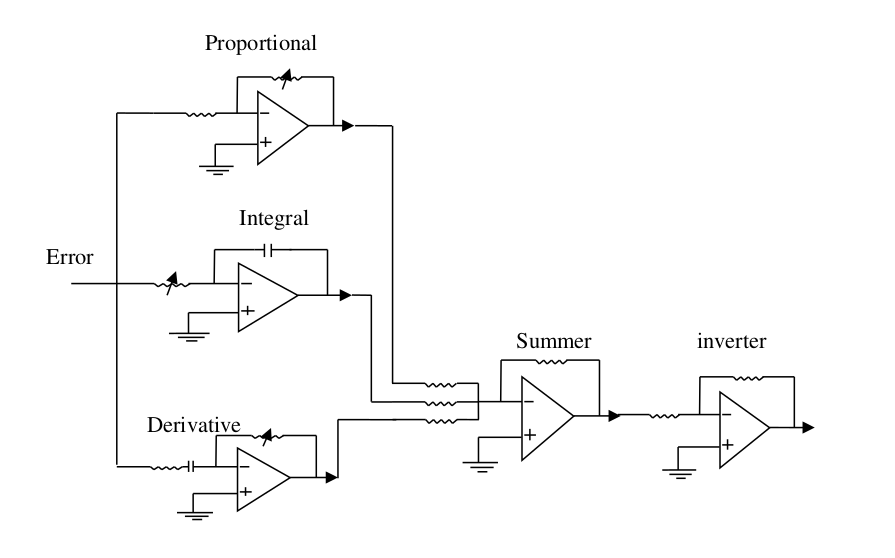
\includegraphics[width=0.6\linewidth]{2Grundlagen/13PID.png}
    \caption{Schematische Darstellung eines PID-Regler. Quelle: \cite[p.~18]{SwainBaid2014}}
    \label{fig:dcdc_converter}
\end{figure}
